\documentclass[12pt]{article}
\usepackage{times}
% increasing margins somewhat to make room for notes
\usepackage[lmargin = 4cm, rmargin = 4cm, tmargin = 2.5cm, bmargin = 2.5cm]{geometry}
\setlength{\marginparwidth}{3.5cm} % make todonotes wider
\usepackage[UKenglish]{babel}
\setlength{\parindent}{0cm}
\usepackage[textsize=tiny]{todonotes}
\usepackage{graphicx}
\newcommand{\todoleft}[1]{{\reversemarginpar \todo{#1}}}

%%%%%%%%%%%%%%%%%%%%%%%%%%%%%%%%%%%%%%%%%%%%%%%%%%%%%%%%%%%%%%%%%%
\begin{document}

\title{Thesis Outline}
\author{Lukas Prader}
\date{}
\maketitle

\section{Introduction}
(citations missing)

%% I compiled this using git-latexdiff (https://gitlab.com/git-latexdiff/git-latexdiff) just to show you how you can get a view of document changes in the rendered PDF.
%% compilation commands:
%% git latexdiff --latexmk --main outline.tex HEAD -- # to compile the current working directory against the last commit
%% git latexdiff --latexmk --main outline.tex HEAD~1 HEAD # to compile the latest commit against the one before
%% you can also refer to specific commit sha hashes

The topic of invasive species has become more and more important, even more so with recent changes in climate and habitats due to human influence.
In order to deal with invasive species and the impact they can have on existing ecosystems, species distribution models (SDMs) have been used to predict the potential habitat and with that the threat of an emerging invasive species.
\todo{This jumps quite quickly to a pretty technical topic, it will need more explanation}
Especially time-partitioned models can provide more insight into the process of invasion. 
Ensemble models are often used in applications where models are projected, since aspects of different modelling approaches can be combined to hopefully gain a more complete model of the species distribution. 

There are certain challenges when using SDMs in invasive research though. 
For example, the invading species is usually not currently in equilibrium with its environment, leading to underestimations of the final niche occupied. 
A similar difficulty is modelling the invaded range with data from a species native range since the native niche can be quite different from the realized invaded niche.

\todoleft{I think, that since your thesis has two goals (understanding H axyridis, but also building a cool model), you can go into more detail on the modelling approach, why it is good, etc in the introduction. The specifics you will still save for methods}
Nonetheless, SDMs are frequently used in trying to predict the spread of invasive species, which is why it is important to gain a better understanding of invasion processes and an SDM's ability to accurately represent it.

\todo{Good start here. Of course eventually your thesis will need quite a bit of background info on the invasion especially}
\textit{Harmonia axyridis}, also known as the harlequin or Asian lady beetle, is an invasive species already established in non-native habitats all around the world.
The invasion process has already been studied extensively and there have been SDMs modelling the invaded range in Europe as well, though mostly on a national scale. 

\todoleft{Good, but I think this needs to be expanded. In particular, the choice of modelling approach needs to be justified in the objectives. What is it that you want to accomplish with this iterative approach? What can we learn from it that we couldn't from a normal ensemble model?}
One goal of this thesis is to look into the limitations of models built early in the invasion process of a species. 
By iterating over the years of the invasion, model performance can be evaluated with consideration to the current state of invasion.
Computing the occupied niche separately for each year also provides more insight into the invasion process and might help to understand modelling limitations for certain years.

\newpage
\section{Methods}
(citations missing)
\subsection{Datasets}
In order to also have some kind of influence of the human nature of first introduction, land cover data was used from the Copernicus Land cover Classification dataset with yearly resolution starting from 2002 up to 2020.

All traditional 19 bioclim variables were obtained from the CHELSA V2.1 climatologies datasets too, using the 1981-2010 time frame for all years from 2002 to 2010 as well as the MPI-ESM 1.2 ssp370 scenario 2011-2040 for all years from 2011 to 2022. 
For occurrence data, all global occurrences of \textit{Harmonia axyridis} were downloaded from the GBIF database.

\subsection{Data preparation}
All bioclim and land cover layers were resampled to a matching resolution of 30 arc seconds and cropped to two spatial extents, Europe and the presumed native range referencing (Orlova-Bienkowskaja, Ukrainsky \& Brown, 2015).

The presence-only points from GBIF were subset to the afore mentioned spatial extents and then checked for missing values for latitude, longitude, year or coordinate uncertainty. 
No occurrences after 2022 were used, also no points with a coordinate uncertainty larger than 1 km. 
In Europe, the initial cut off year for presences was 1991, since this is the year of in vasion according to the EASIN website.
Afterwards, using the library `CoordinateCleaner`, all remaining data points were again checked for common errors or biases in the respective subset.
To prepare the data for modelling, pseudoabsences were generated for each year. 
For this, the subset of a specific year was taken and used to generate pseudo-absences limited to a radius around the occurrence points.
For each presence point, a buffer circle was generated with a maximum distance of 18 km. This buffer circle also excluded any area closer than 1 km to any presence point of any year to limit contradiction in environmental space.

\subsection{Model building}
For each year, the following Models were computed: General Linear (GLM), General Additive (GAM), Boosted Regression Trees (BRT) and Maximum Entropy (MAXENT).  
A model for a specific year always included all points from past years as well.
The iterative models that were built use only data points from Europe, though there was one model created only with native occurrences and predicted for each year in Europe.
For all used occurrence points prior to 2002 and after 2020, the land cover data of 2002 or 2020 was used as a substitute.
\todo{Hmm, yes, that's a challenge, especially if land use is changing quickly. I guess for the most part it is not, but maybe for asia?}
(necessary for after 2020 if only for verification?)

\todo{This will also need more detail}
Variance inflation factors were used to select the variables used for model building. 
For this, a GLM was computed only using Europe data from 2002.
This model included all 19 bioclim variables and their squared values as separate variables.
For land cover variables, a PCA was computed from the 2002 data.
PCA axes were included in the model until a cut off of 80\% of explained variance was reached.
Variance inflation factors were computed for this GLM and the variable with the highest VIF was dropped until none of the remaining variables had a VIF greater than 10. Quadratic versions of bioclim variables were always dropped before their linear counterparts, even if their VIF was lower.

\subsection{Analysis}
\todo{Following year is clear enough, but what's the justification for testing the models against 2022? This would seem like it should automatically prefer SDMs build on current data, because there has been more time for change since 2002?}
\todo{Explain occupied niche and how you computed it; a figure might also be helpful}
All SDM models of each year were tested for their accuracy on predicting the occurrences of the following year and the final year of 2022. 
For each year, the occupied niche was also computed by running a PCA analysis on the bioclim variables. The niche can then be visualized by plotting a dynamic occurrence density grid for the first two PCA axes(Broennimann et al. 2011). 

\begin{figure}[h]
\centering
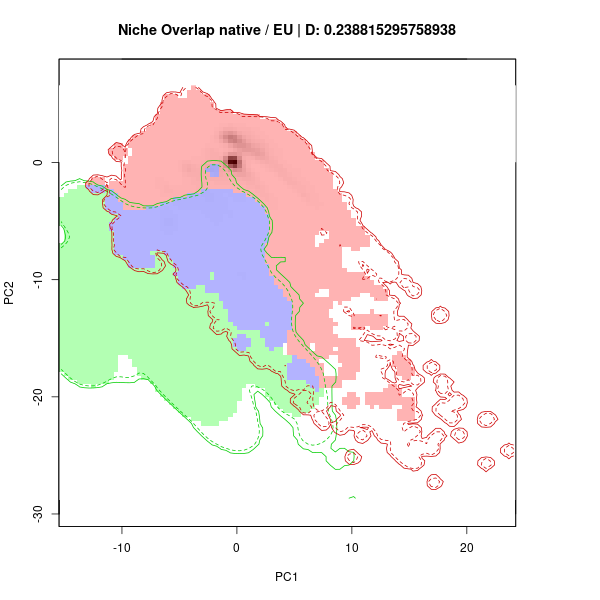
\includegraphics[width = 0.6 \linewidth]{pictures/as-eu-niche.png}
\caption{\label{fig:as-eu-niche} Density grid plot of the bioclimatic niches for the native and invaded European range of \textit{Harmonia axyridis}.}
\end{figure}

\end{document}